\section{Parallel Transport \& Curvature}

\subsection{Parallelity of vector fields}
\begin{definition}
  Let $(M, \mathcal{O}, \mathcal{A}, \nabla)$ be a smooth manifold with connection $\nabla$.
  \begin{enumerate}
    \item[(1)] A vector field $X$ on $M$ is said to be \textbf{parallely transported} along a smooth curve $\gamma: \mathbb{R} \to M$ if 
      \begin{equation}\label{eq:parallelTransport}
        \boxed{\nabla_{v_{\gamma}} X = 0}
      \end{equation}
      To make explicit, how this equation applies along the curve, we may state
      \begin{equation*}
        \left(\nabla_{v_{\gamma, \gamma(\lambda)}} X\right)_{\gamma(\lambda)} = 0
      \end{equation*}
    \item[(2)] A slightly weaker condition is ``\textbf{parallel}'' if, for $\mu : \mathbb{R} \to \mathbb{R}$,
      \begin{equation}
        \boxed{\left(\nabla_{v_{\gamma, \gamma(\lambda)}} X\right)_{\gamma(\lambda)} = \mu(\lambda) X_{\gamma(\lambda)}}
      \end{equation}
  \end{enumerate}
\end{definition}

\textit{Remarks: Even though \textbf{parallely transported} sounds like an action, it is a property.}

\subsection{Autoparallely transported curves}
\begin{definition}
  A curve $\gamma: \mathbb{R} \to M$ is called \textbf{autoparallely transported} if 
  \begin{equation}
    \boxed{\nabla_{v_{\gamma}}v_{\gamma} = 0}
  \end{equation}
\end{definition}

\textit{Remarks: Sometimes, this curve is called an autoparallel curve. But we wish to call a curve autoparallel if $\nabla_{v_{\gamma}}v_{\gamma} = \mu v_{\gamma}$.}

\subsection{Autoparallel equation}
Express $\nabla_{v_{\gamma}} v_{\gamma} = 0$ in terms of chart representation.
\begin{align*}
0 & = \left(\nabla_{v_{\gamma}} v_{\gamma}\right) \\
& = \left(\nabla_{\left(\dot{\gamma}^m_{(x)} \cibasis{x^m}\right)} \dot{\gamma}^n_{(x)} \cibasis{x^n}\right) && \text{ remember that } \gamma^m_{(x)} := x^m \after \gamma \\
& = \dot{\gamma}^m \left(\nabla_{\left(\cibasis{x^m}\right)} \dot{\gamma}^n\right) \cibasis{x^n} + \dot{\gamma}^m \dot{\gamma}^n \left(\nabla_{\left(\cibasis{x^m}\right)} \cibasis{x^n}\right) && \text{x index is understood, hence suppressed} \\
& = \dot{\gamma}^m \left(\cibasis{x^m} \dot{\gamma}^n\right) \cibasis{x^n} + \dot{\gamma}^m \dot{\gamma}^n \left(\nabla_{\left(\cibasis{x^m}\right)} \cibasis{x^n}\right) && \text{} \\
& = \dot{\gamma}^m \left(\cibasis{x^m} \dot{\gamma}^q\right) \cibasis{x^q} + \dot{\gamma}^m \dot{\gamma}^n \left(\Gamma\indices{^{q}_{nm}} \cibasis{x^q}\right) && \text{change of index in 1st term} \\
& = \left(\dot{\gamma}^m \cibasis{x^m} \dot{\gamma}^q + \dot{\gamma}^m \dot{\gamma}^n \Gamma\indices{^{q}_{nm}}\right) \cibasis{x^q} && \text{} \\
& = \left(\ddot{\gamma}^q + \dot{\gamma}^m \dot{\gamma}^n \Gamma\indices{^{q}_{nm}}\right) \cibasis{x^q} && \text{TODO: show that 1st term is 2nd derivative}
\end{align*}

%\begin{frame}
%\begin{figure}
%\label{fig:L8_2ndDerivativeDerivation}
%\centering
%\begin{align*}
%\dot{\gamma}^m \cibasis{x^m} \dot{\gamma}^q & = \left(x^m \after \gamma\right)^\prime \cdot \partial_m\left(\dot{\gamma}^q \after x^{-1}\right)
%\end{align*}
%\caption{Second derivative of a curve}
%\end{figure}
%\end{frame}

In summary:
\begin{equation}\label{Eq:L8_autoParallelTransportChartExpression}
\boxed{\ddot{\gamma}^q_{(x)}(\lambda) + (\Gamma_{(x)})\indices{^{q}_{mn}}(\gamma(\lambda)) \dot{\gamma}^m_{(x)}(\lambda) \dot{\gamma}^n_{(x)}(\lambda) = 0}
\end{equation}
Eq. (\ref{Eq:L8_autoParallelTransportChartExpression}) is the chart expression of the condition that $\gamma$ be autoparallely transported.

\textbf{Example:} (a) In Euclidean plane having a chart $(U = \mathbb{R}^2, x = id_{\mathbb{R}^2})$, $\ccfx{i}{jk}{(x)} = 0 \\
\implies \ddot{\gamma}_{(x)}^m = 0 \implies \gamma_{(x)}^m (\lambda) = a^m \lambda + b^m$, where $a,b \in \mathbb{R}^d$.

(b) Consider the round sphere $(S^2, \mathcal{O}, \mathcal{A}, \nabla_{round}$), i.e., the sphere $(S^2, \mathcal{O}, \mathcal{A})$ with the connection $\nabla_{round}$. Consider the chart $x(p) = (\theta, \phi)$ where $\theta \in (0,\pi)$ and $\phi \in (0, 2\pi)$. In this chart $\nabla_{round}$ is given by
\begin{align*}
\ccfx{1}{22}{(x)}\left(x^{-1}(\theta,\phi)\right) & := - \sin\theta \cos\theta \\
\ccfx{2}{12}{(x)}\left(x^{-1}(\theta,\phi)\right) = \ccfx{2}{21}{(x)}\left(x^{-1}(\theta,\phi)\right) & := \cot\theta
\end{align*}
All other $\Gamma$s vanish. Then, using the sloppy notation (familiar to us from classical mechanics) i.e., $x^1(p) = \theta(p)$ and $x^2(p) = \phi(p)$, the autoparallel equation is
\begin{equation*}
 \left.\begin{aligned}
\ddot{\theta} + \ccf{1}{22} \dot{\phi}\dot{\phi} &= 0 \\
\ddot{\phi} + 2 \ccf{2}{12} \dot{\theta}\dot{\phi} &= 0
       \end{aligned}
 \right\} \implies
\begin{split}
\ddot{\theta} - \sin\theta \cos\theta \dot{\phi}\dot{\phi} &= 0 \\
\ddot{\phi} + 2 \cot\theta \dot{\theta}\dot{\phi} &= 0 \\
\end{split}
\end{equation*}
It can be seen that the above equations are satisfied at the equator where $\theta(\lambda) = \pi/2$, and $\phi(\lambda) = \omega\lambda + \phi_0$ (running around the equator at constant speed $\omega$). Thus, this curve is autoparallel. However, $\phi(\lambda) = \omega\lambda^2 + \phi_0$ wouldn't be autoparallel.

\subsection{Torsion}
Can we use $\nabla$ to define tensors on $(M,\mathcal{O},\mathcal{A},\nabla)$?

\begin{definition}
The \textbf{torsion} of a connection $\nabla$ is the $(1,2)$-tensor field
\begin{equation}
  \boxed{T(\omega,X,Y) := \omega(\nabla_X Y - \nabla_Y X - [X,Y])}
\end{equation}
where $[X,Y]$, called the commutator of $X$ and $Y$ is a vector field defined by $[X,Y]f:= X(Yf) - Y(Xf)$.
\end{definition}

\begin{proof}
We shall check that $T$ is $C^{\infty}$-linear in each entry.
\begin{align*}
T(f\omega, fX, Y) & = f\omega(\nabla_{X} Y - \nabla_Y (X) - [X,Y]) \\
& = fT(\omega, X, Y) \\
T(\omega + \psi, X, Y) & = (\omega + \psi)(\nabla_{X} Y - \nabla_Y (X) - [X,Y]) \\
& = T(\omega, X, Y) + T(\psi, X, Y) \\
T(\omega, fX, Y) & = \omega(\nabla_{fX} Y - \nabla_Y (fX) - [fX,Y]) \\
& = \omega(f\nabla_{X} Y - (\nabla_Y (f))X - f(\nabla_Y X) - [fX,Y]) \\
& = \omega(f\nabla_{X} Y - (Yf)X - f(\nabla_Y X) - [fX,Y]) \\
\text{But } [fX,Y]g & = fX(Yg) - Y(fX)g = fX(Yg) - (Yf)(Xg) - fY(Xg) \implies [fX,Y] = f[X,Y] - (Yf)X \\
\therefore T(\omega, fX, Y) & = \omega(f\nabla_{X} Y - (Yf)X - f(\nabla_Y X) - f[X,Y] + (Yf)X) \\
& = \omega(f\nabla_{X} Y - f(\nabla_Y X) - f[X,Y]) \\
& = f\omega(\nabla_{X} Y - (\nabla_Y X) - [X,Y]) = fT(\omega,X,Y) \\
\text{Further, } T(\omega,X,Y) & = - T(\omega,Y,X), \text{ which means scaling in the last factor need not be checked separately.} \\
\end{align*}
Additivity in the last two factors can also be checked.
\end{proof}

\begin{definition}
  A $(M, \mathcal{O}, \mathcal{A}, \nabla)$ is called torsion-free if the torsion of its connection is zero. That is, $T = 0$.
\end{definition}

In a chart 
\begin{align*}
  T\indices{^i_{ab}} := T\left(dx^i, \cibasis{x^a}, \cibasis{x^b}\right) & = dx^i (\dots) = \ccf{i}{ab} - \ccf{i}{ba} = 2 \ccf{i}{[ab]}
\end{align*}

From now on, in these lectures, we only use torsion-free connections. 

\subsection{Curvature}

\begin{definition}
  \textbf{Riemann curvature} of a connection $\nabla$ is the $(1,3)$-tensor field
\begin{equation}
  \boxed{Riem(\omega,Z,X,Y) := \omega(\nabla_X \nabla_Y Z - \nabla_Y \nabla_X Z - \nabla_{[X,Y]} Z)}
\end{equation}
\end{definition}
\begin{proof}
  It can be shown that $C^{\infty}$-linear in each slot. This has been left as an exercise to the reader.
\end{proof}

\textbf{Algebraic relevance of $Riem$:} We ask whether there is difference in applying the two directional derivatives in different order, i.e. \\
$\nabla_X \nabla_Y Z - \nabla_Y \nabla_X Z = Riem(\cdot,Z,X,Y) + \nabla_{[X,Y]} Z$ \\
In one chart $(U,x)$, denoting $\nabla_{\cibasis{x^a}}$ by $\nabla_a$, \\
$\left(\nabla_a \nabla_b Z \right)^m - \left(\nabla_b \nabla_a Z \right)^m = Riem\indices{^m_{nab}}Z^n + \nabla_{\underbrace{\left[\cibasis{x^a},\cibasis{x^b}\right]}_{=0,\text{ since they commute}}} Z$ \\
As the last term vanishes, we can see how the $Riem$ tensor components contain all the information about how the $\nabla_a$ and $\nabla_b$ fail to commute if they act on a vector field. If they act on a tensor field, there are several terms on RHS like the one term above; if they act on a function, of course they commute. Being a tensor, $Riem$ vanishes in all coordinate systems if it vanishes in one coordinate system, as it does in flat spaces.

\textbf{Geometric significance of $Riem$:} 
\begin{SCfigure}[5][h]
\label{fig:L8_Riem_Geometric_meaning}
  \centering
    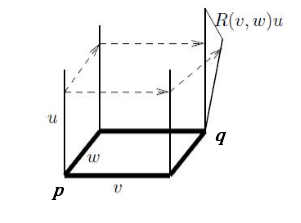
\includegraphics[width=0.3\textwidth]{8_Riem_Geometric_meaning}
    \caption{If we parallel transport a vector $u$ at p to q along two different paths $vw$ and $wv$, the resulting vectors at q are different in general. If, however, we parallel transport a vector in a Euclidean space, where the parallel transport is defined in our usual sense, the resulting vector does not depend on the path along which it has been parallel transported. We expect that this non-integrability of parallel transport characterizes the intrinsic notion of curvature, which does not depend on the special coordinates chosen. \textit{From an answer of Sepideh Bakhoda~\cite{mse465672} on \url{http://math.stackexchange.com/q/465672}}}
\end{SCfigure}

For small $v$ and $w$, if $T = 0$, $(\delta u)^m = Riem\indices{^m_{nab}} v^a w^b u^n + \mathit{O}(v^2w,vw^2)$.
